\section{Data Sources and Sample Construction}\label{sec:data}

\subsection{Official provenance and collection}\label{sec:data-source}
The analysis uses HKJC fixture pages to identify local meetings and HKJC local-results pages to obtain race metadata, runner performance, WIN odds, and dividend tables\cite{hkjcfixtures,hkjcresults}. Collection covers September--July seasons beginning in 2021 and ending in 2026. The fixture parser records date, racecourse, season, and the scheduled number of races. The results parser extracts class and distance text, rating band, going, course configuration, purse, placing, horse number and identifier, jockey, trainer, carried weight, declared body weight, draw, running position, finish time, and displayed WIN odds. The exact WIN dividend per HK\$10 is joined to the winning horse from the official dividend table rather than inferred solely from rounded displayed odds.

The collection was executed on 19 November 2026 with retry logic, local compressed-page caching, and a manifest of request outcomes. There are 444 scheduled meeting--course records, \num{4248} scheduled races on those fixture pages, and \num{4214} archived result races. The difference of 34 races occurs at eight meetings for which the archive contains no result for some or all scheduled races; four of those meetings have no collected result race. This is a coverage difference, not a hidden modeling exclusion. The collector recorded zero request errors across \num{4703} candidate race URLs, including harmless requests beyond the final race number at a meeting. All numerical analysis is based on races for which an official result page was actually retrieved.

\subsection{Cleaning and quality assurance}\label{sec:data-cleaning}
The raw panel contains \num{51553} result rows. Of these, 404 carry HKJC withdrawal codes (WV, WV-A, WX, WX-A, or WXNR) and lack both draw and final WIN odds. An initial audit showed that treating these rows as starters would unnecessarily exclude 383 otherwise valid races and distort field sizes and market probabilities. They are therefore removed before any feature construction. The remaining \num{51149} rows are starters. Seven dead heats are excluded from the present likelihood and its direct evaluation because that likelihood assumes exactly one winner per race; these seven races contain 81 starters, leaving the final \num{4207}-race, \num{51068}-runner modeling sample. Their observed results remain available when subsequent historical features are constructed, because those outcomes would legitimately have been known before later races. No additional race is removed for incomplete odds, draw, carried weight, distance, or winner dividend after this processing.

Quality assurance includes structural and numerical checks. Each included race has exactly one winner, between four and 14 starters, complete market prices, a positive official winner dividend, and the core variables needed by the models. Numeric placings are extracted from labels such as ``1 DH'' before dead heats are identified; non-finishing codes remain non-numeric and receive the worst finishing percentile for historical-form calculations. Probability checks after calibration find a maximum absolute race-sum error below $1.2\times10^{-15}$ across validation and test models. Spot checks against cached official pages also confirmed horse numbers, displayed odds, and exact dividends, including cases where the official dividend differs from ten times the rounded displayed odds.

\begin{table}[htbp]
\centering
\caption{Sample-flow audit from fixture schedule to modeling panel}\label{tab:sampleflow}
\small
\begin{tabularx}{\textwidth}{L{7.3cm} R{2.2cm} Y}
\toprule
\textbf{Stage} & \textbf{Count} & \textbf{Interpretation} \\
\midrule
Scheduled meeting--course records & 444 & HKJC fixture records in five seasons. \\
Scheduled races on fixture pages & \num{4248} & Planned race count before archive availability checks. \\
Archived result races collected & \num{4214} & Official races with a parseable result table. \\
Raw runner result rows & \num{51553} & Includes horses subsequently recorded as withdrawn. \\
Withdrawn rows removed & 404 & Non-starters across 383 races; removed before field-size calculation. \\
Starters after withdrawal removal & \num{51149} & Runners eligible for sample inclusion. \\
Dead-heat races excluded & 7 & Single-winner likelihood restriction; 81 starters removed. \\
Final modeling races / starters & \num{4207} / \num{51068} & Complete cases used for chronological analysis. \\
Result meetings represented & 440 & 88 result meetings in each season. \\
\bottomrule
\end{tabularx}
\source{Project collection manifest, coverage table, and sample-exclusion audit.}
\end{table}

\subsection{Chronological partitioning}\label{sec:data-split}
The seasons are partitioned by time rather than randomly sampled. Seasons 2021/22--2023/24 provide \num{2498} training races and \num{29967} runners; 2024/25 provides 847 validation races and \num{10341} runners; and 2025/26 provides 862 test races and \num{10760} runners. Model regularization, the primary trained model, and calibration temperature are selected or fitted using training and validation information only. The test season is evaluated after those decisions. Historical feature accumulation does not reset at season boundaries, because prior-season information would legitimately be available for a future race, but no current or future outcome enters a predictor.

This design sacrifices the simplicity of random cross-validation in exchange for a more realistic forecasting question. Horse, jockey, and trainer populations evolve; class compositions and market behaviour can drift; and the same entities naturally recur across training and test periods. Such recurrence is not itself leakage because only earlier outcomes are used. The principal remaining threat is temporal distribution shift, which cannot be eliminated by splitting. It is assessed indirectly by comparing validation and test metrics and will be examined more fully through rolling-origin experiments in the remaining work.

\begin{table}[htbp]
\centering
\caption{Chronological data partition}\label{tab:split}
\small
\begin{tabular}{L{4.1cm} L{3.2cm} R{2.0cm} R{2.2cm} C{2.3cm}}
\toprule
\textbf{Season(s)} & \textbf{Role} & \textbf{Races} & \textbf{Runners} & \textbf{Result meetings} \\
\midrule
2021/22--2023/24 & Training & \num{2498} & \num{29967} & 264 \\
2024/25 & Validation and calibration & 847 & \num{10341} & 88 \\
2025/26 & Untouched test & 862 & \num{10760} & 88 \\
\midrule
\textbf{Total} & & \textbf{\num{4207}} & \textbf{\num{51068}} & \textbf{440} \\
\bottomrule
\end{tabular}
\end{table}

\begin{figure}[htbp]
\centering
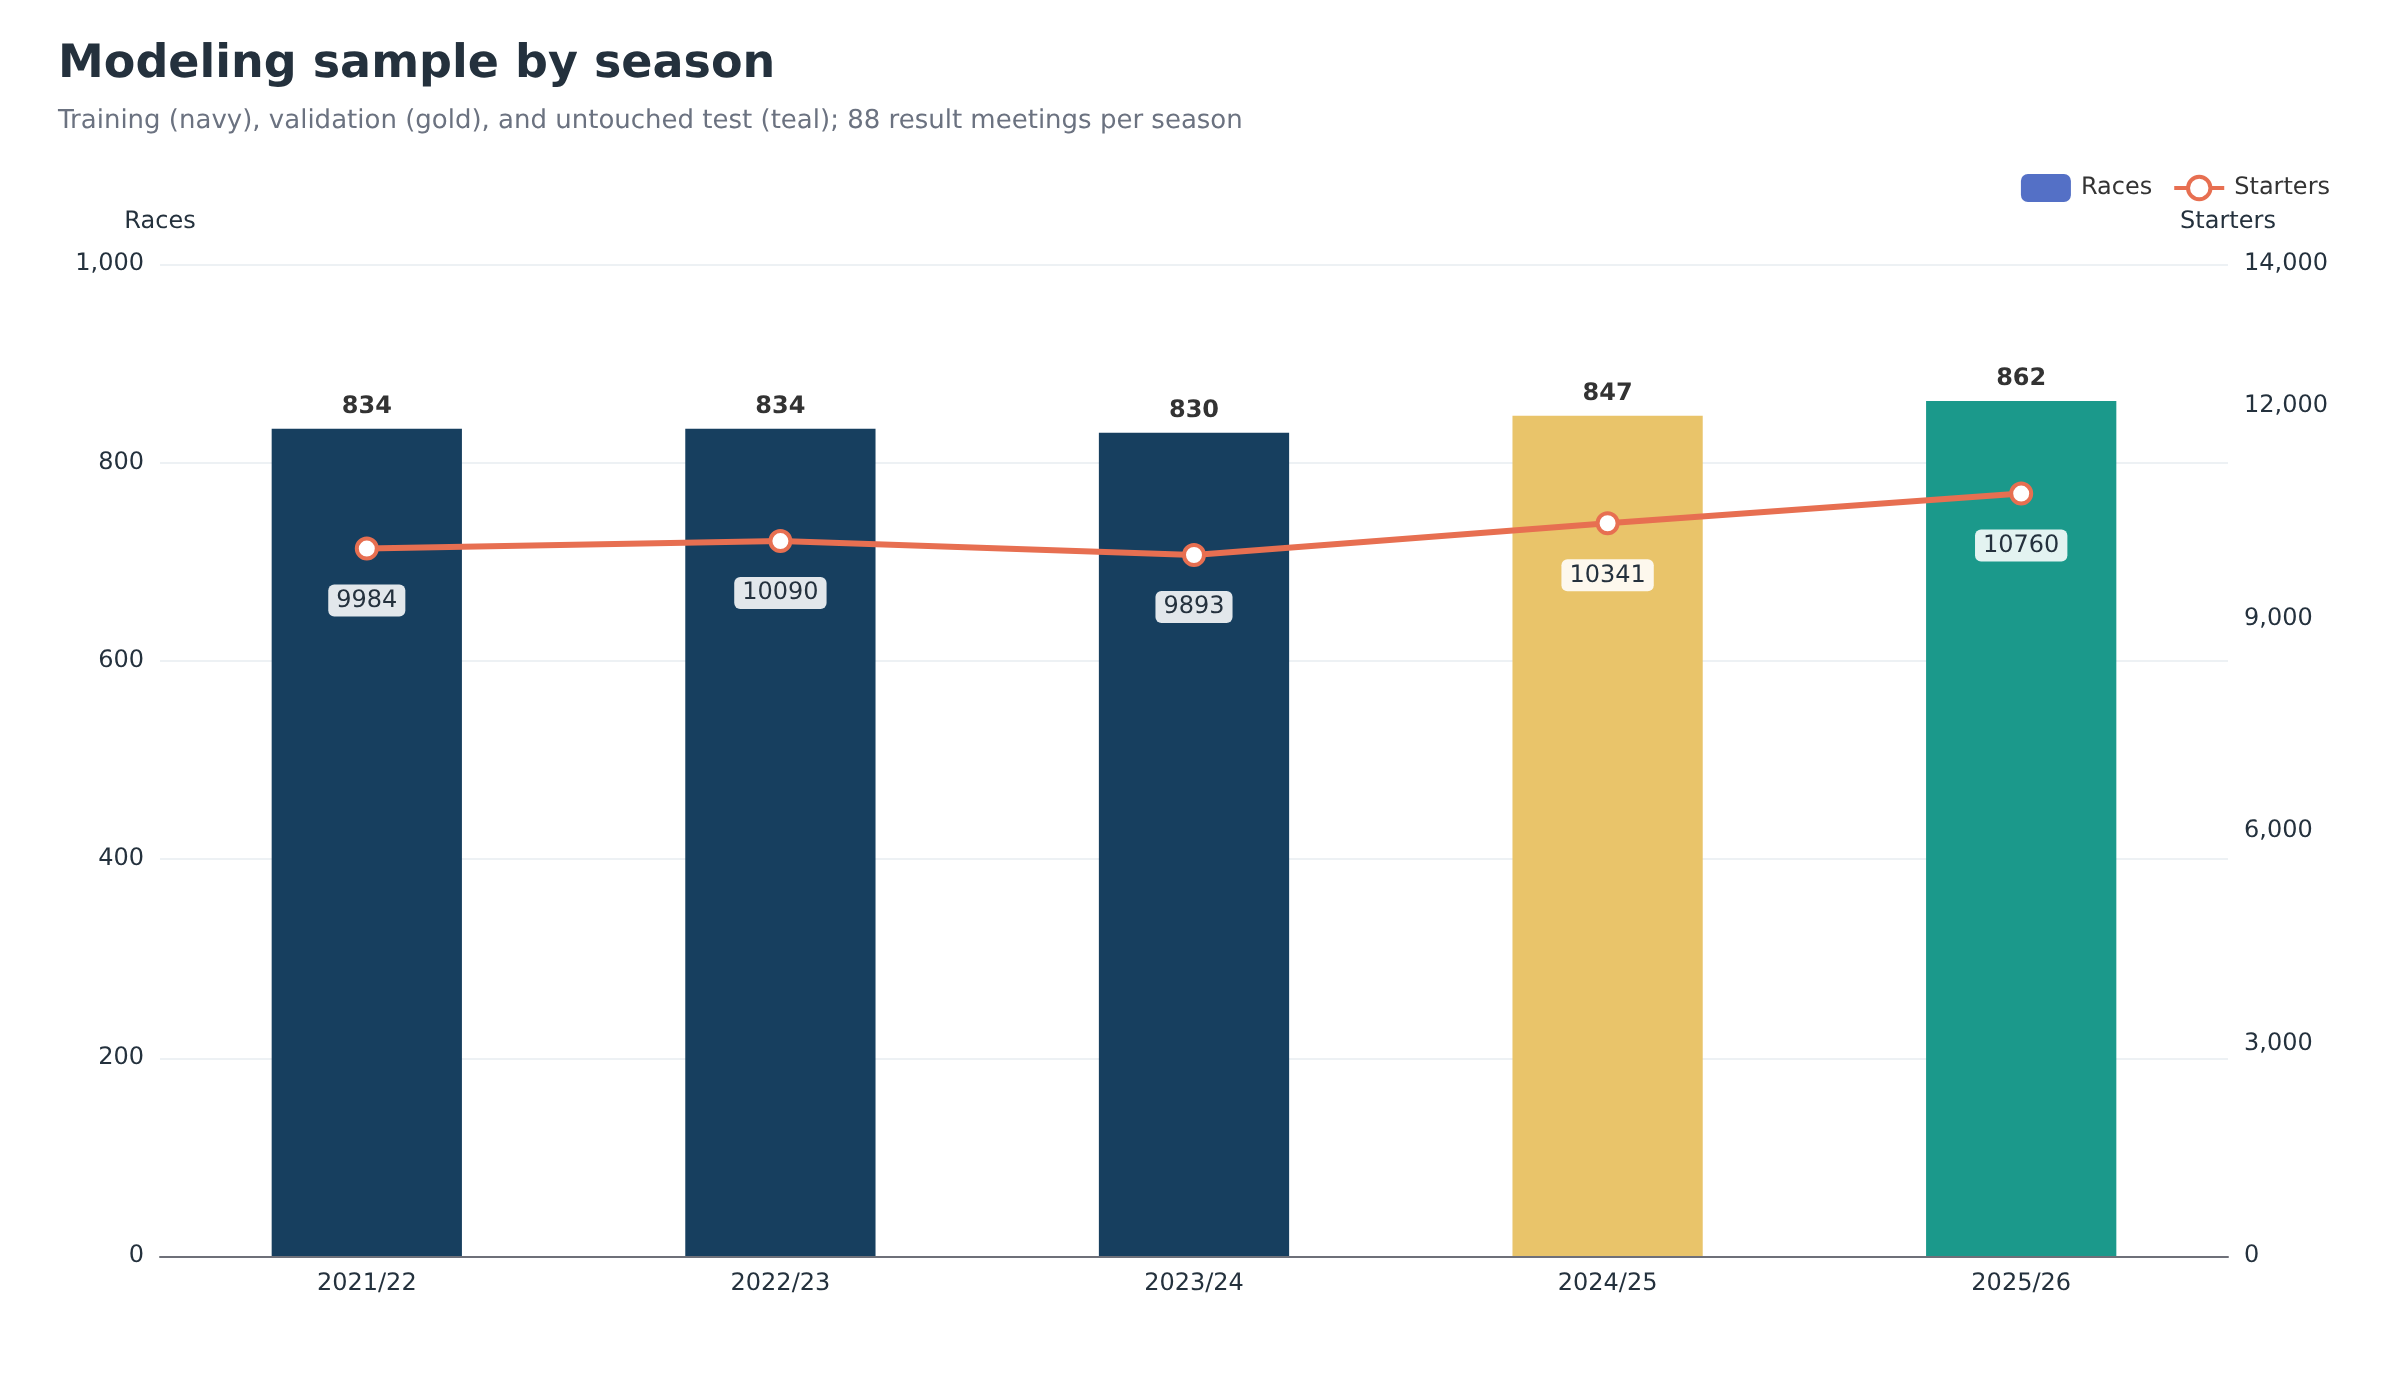
\includegraphics[width=0.96\textwidth]{season_sample.png}
\caption{Season-level modeling sample and chronological roles. Bar labels give races; line labels give starters. The first three seasons form training, 2024/25 is validation, and 2025/26 is the untouched test.}\label{fig:season-sample}
\end{figure}

\subsection{Descriptive characteristics}\label{sec:data-descriptive}
Table~\ref{tab:season-descriptives} shows that the sample is broadly stable in scale but not identical across seasons. Mean field size rises from 11.92 in 2023/24 to 12.48 in the test season, while the average race overround remains close to 1.227--1.228. Here overround is the sum of reciprocal displayed decimal odds within a race, and normalized market probability is each reciprocal divided by that sum. This normalization removes the mechanical scale excess but does not by itself prove calibration or remove dividend rounding. The similarity of overround across seasons makes the chronological comparisons easier to interpret, although it does not rule out changes in other market characteristics.

Observed favourite performance varies across seasons. The single lowest-odds selection, with horse number breaking ties, wins 33.45\% of races in 2022/23 but 28.65\% in 2025/26. These are descriptive frequencies, not by themselves evidence of structural non-stationarity: with roughly 830--860 races per season, sampling uncertainty is material. The variation nevertheless cautions against treating one season's favourite strike rate as a fixed parameter. It also anticipates the distinction between prediction and return: even when favourites win approximately three races in ten, their average price can be insufficient to cover stakes and pool effects. Section~\ref{sec:results-betting} therefore evaluates both outcomes and official-dividend returns.

\begin{table}[htbp]
\centering
\caption{Descriptive statistics by season}\label{tab:season-descriptives}
\small
\begin{tabular}{L{2.1cm} R{1.3cm} R{1.6cm} R{1.6cm} R{1.9cm} R{1.9cm}}
\toprule
\textbf{Season} & \textbf{Races} & \textbf{Mean field} & \textbf{Mean overround} & \textbf{Favourite win rate} & \textbf{Runners} \\
\midrule
2021/22 & 834 & 11.97 & 1.22782 & 28.90\% & \num{9984} \\
2022/23 & 834 & 12.10 & 1.22803 & 33.45\% & \num{10090} \\
2023/24 & 830 & 11.92 & 1.22766 & 29.40\% & \num{9893} \\
2024/25 & 847 & 12.21 & 1.22757 & 32.82\% & \num{10341} \\
2025/26 & 862 & 12.48 & 1.22694 & 28.65\% & \num{10760} \\
\bottomrule
\end{tabular}
\source{Race-level means use one observation per race. Favourite ties are broken by horse number.}
\end{table}
